\JWlone{Methodology}
\label{sec:methods}

%
% ILLUSTRATION
%
\JWltwo{Illustration}
\label{sec:illustration}

This chapter informally illustrates the key ideas and methods proposed by this
thesis. The following chapters contain a more formal bottom--up description that
is rather cumbersome to understand without grasping the overall picture.

The goal is to obliviously evaluate a polynomial by two mutual distrusting
parties. Informally, that means to evaluate a polynomial ($f(x) = \sum a_ix^i$)
where the first party chooses $f$ and the second party chooses $x$. It is
crucial that neither party learns the choice of the other party. The naive and
simple solution is to instruct a trusted third party to evaluate the
polynomial---provided by the first party---at the grid point $x$ provided by the
second party. Of course, this solution is just as simple as insecure because the
third party could reveal its secrets at any time.

The thesis expresses the general polynomial as affine functions that evaluate
parts of the complete function. The entirety of the affine functions exactly
represents the original polynomial. The process is based on dividing the input
polynomial into affine functions, because \JWdefn{Oblivious Affine Function
Evaluation} {OAFE} \cite{davidgoliath} are used as the main building block.
Every OAFE enables one party to choose an affine function that another party can
evaluate obliviously. The OAFE guarantees that the second party does not learn
the affine function and that the first party does not learn the node at which
the second party evaluated the function. Additionally OAFE guarantees every
linear function can only be evaluated once. To maintain the security property
for the input polynomial, neither party should be able to learn anything from
intermediate results.

The role both parties play differs heavily: The first party---usually named
\JWpOne{}---is in possession of the polynomial to evaluate and sets up the
OAFEs.  The second party---usually named \JWpTwo{}---is less powerful: It does
only evaluate entities issued by \JWpOne{} and uses the already configured
OAFEs. But in the end, only \JWpTwo{} obtains the result.  Since the OAFEs play
an important role, it is crucial to envision that every OAFE \JWpOne{} generates
can be evaluated by \JWpTwo{} only once. In other words, an OAFE enables some
party to evaluate an affine function at one node and guarantees that no further
evaluations are possible. To prevent a corrupted \JWpOne{} from intercepting
information when \JWpTwo{} evaluates one of the OAFEs, \JWpOne{} is forced to
commit itself to a finite number of OAFEs a priori. \JWpOne{} is also forced to
commit itself to all parameters for all OAFEs. The OAFE implementation from
Döttling, Kraschewski and Müller--Quade\cite{davidgoliath} realizes the OAFE
functionality on exactly one tamper--proof hardware token, that has to be
physically sent to the other party. Because the OAFE functionality realizes all
OAFEs together, \JWpOne{} needs to commit itself to the OAFE configuration a
priori. \JWpOne{} configures all OAFEs before \JWpTwo{} even starts the process.

All following steps will be performed by \JWpTwo{} alone, no further interaction
with \JWpOne{} is necessary. An honest \JWpTwo{} acts completely
deterministically and will receive the function's final evaluated value $f(x)$.
The following process dividing the function in smaller parts usually uses the
term \emph{(arithmetic) circuit}. The term circuit means a rooted evaluation
tree (e.g., figure \ref{fig:sample-poly}) of a function where the leaf nodes
contain values or inputs and the inner nodes---called (arithmetic) gates---do
arithmetic operations.

The approach pursued here is to divide the arithmetic circuit that equals the
overall function to smaller sub--circuits. Each sub--circuit can be composed of
arithmetic gates and other sub--circuits. \JWpTwo{} is commissioned to evaluate
each sub--circuit to an intermediate value. \JWpTwo{} then stores all
intermediate values since they are used to compute the following sub--circuits.
Whenever one sub--circuit $A$ contains a node that is another sub--circuit $B$,
this node gets replaced by the intermediate output value of $B$ before
evaluating $A$.  Obviously the intermediate values are a potential security
threat: A passively corrupted \JWpTwo{} could try to derive information from
these intermediate results. An actively corrupted \JWpTwo{} could additionally
try to modify the intermediate values and gain supplemental information out of
that. To not directly reveal the value of an evaluated sub--circuit the
intermediate values have to be \emph{encrypted}. To be able to identify an
illicit forgery the overall evaluation has to fail when an attacker tries to
illicitly modify an intermediate result. In this thesis, the intermediate values
are tuples of two values. The decryption of both values represents---when
well--formed---the same value. The gain of this technique is that an attacker
cannot change the value and preserve the well--formedness without knowing the
encryption keys. Any change to one (or both) tuple values causes the
intermediate value to be destroyed (formally represented as $\bot$). After
having evaluated the last sub--circuit, its resulting encrypted tuple undergoes
a special procedure revealing the unencrypted scalar result value. Details and
the formal description of the procedures mentioned above can be found in the
following chapters.

\begin{figure}[htb]
  \centering
  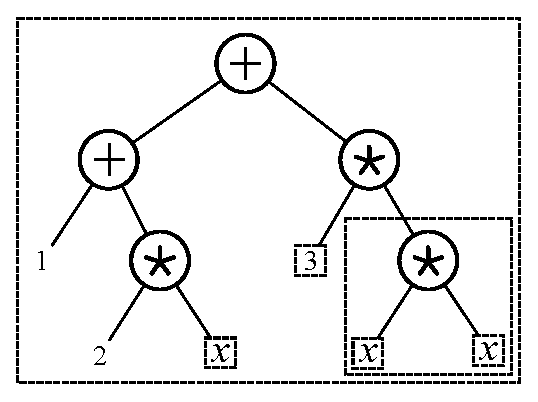
\includegraphics[width=10cm]{images/sample-polynomial.eps}
  \caption{Circuit encoding the polynomial $1 + 2x + 3x^2$ including its
    (sub--)circuits (dashed boxes)}
  \label{fig:sample-poly}
\end{figure}

The overall process is very straightforward: \JWpOne{} analyzes the polynomial
and transforms it into a circuit (the entire figure \ref{fig:sample-poly}). This
circuit is then divided to sub--circuits (the boxes bounded by dashed lines).
All the sub--circuits are then encoded in a way that \JWpTwo{} cannot learn
anything private to \JWpOne{}. To achieve that, \JWpOne{} sets up an OAFE and
hands the OAFE along with a description of the sub--circuits to \JWpTwo{}.
After sending the circuits and the OAFE functionality, \JWpOne{} can shut down
because it is no longer needed in the process. As soon as \JWpTwo{} receives the
sub--circuit description and the OAFEs, it starts the evaluation, one
sub--circuit after the other. To discuss the evaluation the sample polynomial $1
+ 2x + 3x^2$ (see figure \ref{fig:sample-poly}) is used in the following. In the
whole procedure, \JWpTwo{} should not learn the coefficients ($a_0$, $a_1$ and
$a_2$) of the polynomial $a_0 + a_1x + a_2x^2$ but is able to learn the degree
of the polynomial. The first step for \JWpTwo{} is to evaluate the sub--circuit
only containing $x$.  This is in fact only one sub--circuit that appears three
times in the figure.  The next step would be to evaluate the sub--circuit only
encoding $3$ (remember, not learning the value $3$!), then the sub--circuit
encoding $x^2 (= x \cdot x)$ and finally the overall circuit that encodes $1 +
2x + 3x^2$.  Usually and as in the example above, the sub--circuits are of
maximal size. Notably, a sub--circuit can only contain multiplications that only
depend on either constants or stored intermediate values.

To simplify the analysis of the different parts and to show the
modularity, special terms are used throughout in this thesis. A mapping from the
informal terms used above and the terms used otherwise (and defined in the
following chapters) follows:

In the informal illustration above, the encoded tuples played an important role.
They represented values and the sub--circuits evaluated to these encrypted
tuples. In fact, the sub--circuits are also twofold, they have a left and a
right side that eventually evaluate to two values: Both sides of the encrypted
tuple. For technical reasons, the two sides of the circuits and the tuples are
often handled apart. They still represent the same value encrypted with
different keys. For this reason the terms below all exist in two forms, the
\emph{Double} form (such as \emph{Double Randomized Affine Encoding}) and the
regular form (such as \emph{Randomized Affine Encoding}). At some point in the
processing, they are split syntactically, two regular entities are just the same
as one Double entity. The difference is mainly the same as naming tuple
$\widetilde{a} = (\widetilde{a_l}, \widetilde{a_r})$ \emph{Double Value} and
$\widetilde{a_l}$ and $\widetilde{a_r}$ \emph{Value}s.

\begin{itemize}

  \item The intermediate values that are encrypted twofold are named
    \emph{Double Randomized Affine Values} (DRAV), defined in chapter
    \ref{def:DRAV}.

  \item The encodings of sub--circuits are called \emph{Double Affine Randomized
    Encodings} (DRAE) and \emph{Randomized Affine Encodings} (RAE) defined in
    chapter \ref{def:DRAE}. Each (D)RAE is assigned to an intermediate variable
    that occurs in the subsequent (D)RAEs. A (D)RAE is a specification of
    calculations that have to be performed until obtaining the (D)RAEs result
    value. For the (D)RAC, the result value is just an intermediate
    value that a sub--circuit evaluated to.

  \item The overall circuit representing exactly one function is named
    \emph{Double Affine Randomized Circuit} (DRAC) or \emph{Affine Randomized
    Circuit} (RAC) defined in chapter \ref{def:DRAC}. A DRAC is the collectivity
    of DRAEs each assigned to intermediate variables storing their result
    values.

\end{itemize}


%
% DEFINITIONS
%
\JWltwo{Definitions}
\label{sec:rae-definitions}

This chapter defines important entities that are used in the following chapters.

% Field K
\JWlthree{Field $\mathbb{K}$}
\label{sec:field}

\label{def:field} Throughout this thesis, $\mathbb{K}$ represents an arbitrary
large finite field, such as $\mathbb{F}_{2^{256}}$.  When not mentioned
otherwise, this thesis assumes the field $\mathbb{F}_{2^{256}}$ specified by the
irreducible polynomial $1 + x^2 + x^5 + x^{10} + x^{256}$.


% OAFEs
\JWlthree{Oblivious Affine Function Evaluation}

The main building block of this thesis are \JWdef{Oblivious Affine Function
Evaluation}{OAFE}{s}. More precisely, \emph{Sequential one--time OAFE} as
defined by Döttling, Kraschewski and Müller--Quade \cite{davidgoliath}. The OAFE
functionality enables to sequentially evaluate $n$ affine functions specified a
priori. The OAFE functionality is implemented by the David \& Goliath protocol
\cite{davidgoliath} and exactly one stateful tamper--proof hardware token. In
other words, one party can specify $n$ affine functions and another party will
be able to sequentially evaluate the functions exactly once. The evaluating
party will only learn one evaluation of each function $f_i$ but not their
definition. After all $n$ functions have been evaluated the tamper--proof
hardware token can be physically destroyed.

\begin{align*}
  i \in& \{1, \ldots, n\}\\
%
  f_i(x_i) = &
  a_ix_i + b_i \\
%
  = &
\begin{pmatrix}a_{i,1}\\a_{i,2}\\a_{i,3}\\\vdots\end{pmatrix}x_i +
\begin{pmatrix}b_{i,1}\\b_{i,2}\\b_{i,3}\\\vdots\end{pmatrix}
\end{align*}

\noindent{}For the sake of simplicity, the term \emph{OAFE} is used slightly
different in this thesis: The term \emph{OAFE} is a functionality to evaluate
one affine function. The plural (\emph{OAFEs}) means a set of OAFEs that enable
to evaluate multiple affine functions. Therefore the collectivity of OAFEs as
defined in this thesis can be implemented by one \emph{Sequential one--time
OAFE} functionality as defined by Döttling, Kraschewski and Müller--Quade
\cite{davidgoliath}.


%
% DUAL RANDOMIZED AFFINE VALUES
%
\JWltwo{Dual Randomized Affine Values}
\label{sec:drav}

\JWdef{Dual Randomized Affine Value}{DRAV}{s} are encrypted, signed values
representing a scalar value of the field $\mathbb{K}$. Each DRAV is encrypted
with a pair of \emph{dual keys}. The first dual key, the \emph{static key},
remains the same in the whole DRAC (see chapter \ref{def:DRAC}) generation
procedure and is usually denoted as $(\alpha_l, \alpha_r)$. The second dual key,
the \emph{dynamic key} is a short--lived key, usually represented as $(\beta,
\beta')$. Two DRAVs only share the same dynamic key by chance but always share
the same static key. Encoding a regular value $v \in \mathbb{K}$ as a DRAV
$\widetilde{v}$ is straightforward: For the sake of simplicity this thesis
assumes a function $E(v)$ (also named \emph{universal encoding function}) that
is implicitly parametrized by the static dual key $(\alpha_l, \alpha_r)$ and is
able to generate a new dynamic dual key $(\beta, \beta')$ uniformly at random.
Just like $E(v)$, this thesis also assumes $D(\widetilde{v})$, named the
\emph{universal decoding function}. The universal decoding function is assumed
to be implicitly parametrized by the encryption keys from the context it is used
in. Both functions are defined below.  The universal encoding and decoding
functions only serve the purpose of describing the methodology. In the reality
especially the function $D$ is never called by anyone. That would not even be
possible since only the party in possession of the keys (\JWpOne{}) has the
information to do so but because of the non--interactivity of the protocol,
\JWpOne{} is not active anymore when the second party (not in possession of the
keys, usually named \JWpTwo{}) starts the evaluation. The real protocol encodes
the encryption and decryption into the OAFEs in a way that as soon as \JWpTwo{}
tries to cheat everything eventually becomes uniform randomness. To cheat means
to disrespect the protocol description and to misbehave in any way. The property
to turn everything to uniform randomness as soon as a party tries to cheat is
done using carefully chosen linear functions realized as OAFEs. The setup of
these linear functions assures the addition of uncorrelated uniform randomness
as soon as \JWpTwo{} tries to cheat. One can envision the process as applying a
one--time pad encryption that is only correctly removed if the other party did
not try to cheat. As soon as the second party tries to cheat this resembles the
attempt to undo a one--time pad encryption using another one--time pad. This
clearly leads to a one--time pad encryption which can only be undone using an
unknown one--time pad. The unknown one--time pad is a composition of the
encrypting one--time pad and the one--time pad using which the decryption was
attempted.

\begin{align}
  \label{eqn:one-time-pad}
  \hat{E}(v; \alpha_l, \alpha_r, \beta, \beta') &=
  (\alpha_l \cdot v + \beta, \alpha_r \cdot v + \beta')\\
  %
  E(v) &= \hat{E}(v; \alpha_l, \alpha_r, \beta, \beta') \qquad
  \text{(implicitly knowing the keys)}\nonumber
  %
\end{align}

\noindent{}The values $\beta$ and $\beta'$ are as mentioned above fresh values
uniformly at random. In finite fields $\beta$ and $\beta'$ therefore one--time
encrypt both tuple components, as such a DRAV is one--time pad encrypted.
$\alpha_l$ and $\alpha_r$ are also values uniformly at random but are in
contrast to $\beta$ and $\beta'$ used in for DRAVs throughout the whole
process. The purpose they serve will be discussed in the following chapters.

Notationally, the DRAV encoding a scalar value $v$ is usually denoted as
$\widetilde{v}$. $\widetilde{v}$'s tuple components are usually called
$\widetilde{v_l}$ and $\widetilde{v_r}$: $(\widetilde{v_l}, \widetilde{v_r}) =
\widetilde{v} = E(v)$. Where appropriate, DRAVs are also denoted in a vector
notation $\begin{pmatrix}\widetilde{v_l}\\\widetilde{v_r}\end{pmatrix}
\entspricht (\widetilde{v_l}, \widetilde{v_r}) = E(v)$. The universal decoding
function $D(\widetilde{v})$ is:

\begin{align}
  %
  \hat{D}(\widetilde{v}; \alpha_l, \alpha_r, \beta, \beta') &=
  \begin{pmatrix}
    \frac{\widetilde{v_l} - \beta}{\alpha_l}\\
    \frac{\widetilde{v_r} - \beta'}{\alpha_r}
  \end{pmatrix} \nonumber\\
  %
  \label{eqn:keys-assumed}
\begin{pmatrix}D_l(\widetilde{v})\\D_r(\widetilde{v})\end{pmatrix} &=
  \hat{D}(\widetilde{v}; \alpha_l, \alpha_r, \beta, \beta') \qquad
  \text{(implicitly knowing the keys)}\\
  %
  D(\widetilde{v}) &=
  \left\{
    \begin{array}{l l}
      D_l(\widetilde{v}) & \quad
      \text{if}~D_l(\widetilde{v}) = D_r(\widetilde{v})\\
      \bot & \quad \text{otherwise ($\widetilde{v}$ is non--well--formed)}\\
    \end{array}\right.\nonumber
    %
\end{align}

\noindent{}In equation \ref{eqn:keys-assumed} one can see that the universal
decoding function $D$ assumes context--specific  dual keys $(\alpha_l,
\alpha_r)$ and $(\beta, \beta')$. If an attacker at some point passes a DRAV
that is not expected to be decoded at this point, the decoding will fail and
evaluate to $\bot$. This is evident because $D$ will decode using the dual keys
of the DRAV that was expected to be decoded (see also Lemma
\ref{lem:well-formed-fun-of-dec-fun}).

\begin{lem}
  \label{lem:DRAV-random}

  A party that is not in possession of the encryption (dual) keys will not learn
  anything from a DRAV\@. A DRAV is a tuple consisting of two values uniformly
  at random that is uncorrelated to any other DRAV\@.

\end{lem}
\begin{proof}

  In a finite field, the addition of some value $r$ uniformly at random to
  another value $x \in \mathbb{K}$ is uniformly at random. Therefore $\alpha_l
  \cdot v + \beta$ and $\alpha_r \cdot v + \beta'$ are two values uniformly at
  random if and only if $\beta$ and $\beta'$ are uniformly at random. Per
  definition, every time a DRAV gets encoded, $\beta$ and $\beta'$ are fresh
  uniformly distributed random values. Trivially, a DRAV is therefore
  uncorrelated to any other DRAV\@.

\end{proof}


% WELL-FORMED DRAVs
\JWlthree{Well--Formed DRAVs}
\label{sec:well-formed-DRAV}

A DRAV $\widetilde{v}$ is well--formed iff $D(\widetilde{v}) \neq \bot
\Leftrightarrow D_l(\widetilde{v}) = D_r(\widetilde{v})$. Therefore, if
$D(\widetilde{\chi}) = \bot$, $\chi$ is non--well--formed. Obviously the
well--formedness of a DRAV depends on the encryption keys used to decrypt.
Decoding well--formed DRAVs using any other decoding function will highly likely
lead to $\bot$ because the well--formed DRAV looks non--well--formed to the
other decoding function. Decoding using another decoding does not lead to
$\bot$, iff both DRAVs have the same encryption keys. The probability is
therefore $\frac{1}{2*|\mathbb{K}|}$, $\mathbb{K}$ (see chapter \ref{sec:field}
being the finite field and $|\mathbb{K}|$ its size.

\begin{lem}
  \label{lem:well-formed-fun-of-dec-fun}

  DRAV well--formedness is a function of the keys used to decrypt it.

\end{lem}
\begin{proof}

  Assuming two well--formed DRAVs $\widetilde{a}$ and $\widetilde{b}$. Both
  DRAVs have their respective decoding function $D^a$ and $D^b$ and their
  dynamic dual key (say $(\beta_1, \beta_2)$ for $\widetilde{a}$ and
  $(\beta_3, \beta_4)$ for $\widetilde{b}$). The following equations show
  the decoding of the DRAVs $\widetilde{a}$ and $\widetilde{b}$ with the correct
  keys and the wrong keys.

  \begin{align*}
    %
    D^a(\widetilde{a}) &= D(\widetilde{a}) \qquad\text{(using $\widetilde{a}$'s
    keys)}\\
    %
    D^b(\widetilde{b}) &= D(\widetilde{b}) \qquad\text{(using $\widetilde{b}$'s
    keys)}\\
    %
    a &= D^a(\widetilde{a}) \entspricht
    \begin{pmatrix}
      \frac{(\alpha_l \cdot a + \beta_1) - \beta_1}{\alpha_l}\\
      \frac{(\alpha_r \cdot a + \beta_2) - \beta_2}{\alpha_r}\\
    \end{pmatrix}
    = a\\
    %
    a' &= D^a(\widetilde{b}')
    \entspricht
    \begin{pmatrix}
      \frac{(\alpha_l \cdot b + \beta_3) - \beta_1}{\alpha_l}\\
      \frac{(\alpha_r \cdot b + \beta_4) - \beta_2}{\alpha_r}\\
    \end{pmatrix}
    \entspricht
    \begin{pmatrix}
      b +
      \frac{\beta_3 - \beta_1}{\alpha_l}\\
      b +
      \frac{\beta_4 - \beta_2}{\alpha_r}\\
    \end{pmatrix}
    \stackrel{*}{=} \bot\\
    %
    b &= D^b(\widetilde{b}) \entspricht
    \begin{pmatrix}
      \frac{(\alpha_l \cdot b + \beta_3) - \beta_3}{\alpha_l}\\
      \frac{(\alpha_r \cdot b + \beta_4) - \beta_4}{\alpha_r}\\
    \end{pmatrix}
    = b\\
    %
    b' &= D^b(\widetilde{a}')
    \entspricht
    \begin{pmatrix}
      \frac{(\alpha_l \cdot a + \beta_1) - \beta_3}{\alpha_l}\\
      \frac{(\alpha_r \cdot a + \beta_2) - \beta_4}{\alpha_r}\\
    \end{pmatrix}
    \entspricht
    \begin{pmatrix}
      a +
      \frac{\beta_1 - \beta_3}{\alpha_l}\\
      a +
      \frac{\beta_2 - \beta_4}{\alpha_r}\\
    \end{pmatrix}
    \stackrel{*}{=} \bot\\
    %
    &\JWnegl{}
  \end{align*}

  \noindent{}As shown above, decoding a well--formed DRAV using the wrong
  decoding function leads to $\bot$.

\end{proof}


\begin{lem}
  \label{lem:DRAV-indistinguishable}

  Without knowing the encryption keys, a non--well--formed DRAV is
  indistinguishable from a well--formed DRAV\@.

\end{lem}
\begin{proof}

  From Lemma \ref{lem:DRAV-random} we learn, that a well--formed DRAV only
  consists of two values uniformly at random. From Lemma
  \ref{lem:well-formed-fun-of-dec-fun} we learn, that well--formedness is a
  function of the encryption keys used to eventually decrypt the DRAV\@. Since a
  party that is not in possession of the encryption keys cannot know the
  decryption function, well--formed and non--well--formed DRAVs are
  indistinguishable for a party not in possession of the keys.

\end{proof}


% DIRECT DRAV ARITHMETIC
\JWlthree{Direct DRAV Addition}
\label{sec:DRAV-addition}

This thesis refers to DRAV addition as \emph{direct DRAV addition} because it
has the property to be performable without knowledge of a DRAV's encryption
keys. But (see Lemma \ref{lem:wrong-add}) the addition of DRAVs does not lead to
additional information. Although addition can be performed without the knowledge
of the encryption keys, it will not reveal additional information because the
encryption keys automatically changes. Therefore, the result will only be
well--formed iff the addition was intended by the party in possession of the
keys (see Lemma \ref{lem:well-formed-fun-of-dec-fun}).

\begin{lem}
  \label{lem:DRAV-add}

Additions commissioned by a party in possession of the encryption keys of
well--formed DRAVs lead to well--formed DRAV: $\widetilde{x} =
(\widetilde{x_l}, \widetilde{x_r})$ and $\widetilde{y} = (\widetilde{y_l},
\widetilde{y_r})$ can be added component--wise to $\widetilde{z} =
\left(\widetilde{x_1} + \widetilde{y_1}, \widetilde{x_2} +
\widetilde{y_2}\right)$. The encryption keys for $\widetilde{z}$ will be
$(\alpha_l, \alpha_r)$ and $(\beta_1 + \beta_3, \beta_2 + \beta_4)$ assuming
$\widetilde{x}$ was encrypted with $(\alpha_l, \alpha_r)$ and $(\beta_1,
\beta_2)$ and $y$ was encrypted with $(\alpha_l, \alpha_r)$ and $(\beta_3,
\beta_4)$.

\end{lem}
\begin{proof}

From ($\widetilde{x} = \left(\alpha_l \cdot x + \beta_1,
\alpha_r \cdot x + \beta_2\right)$, $\widetilde{y} = \left(\alpha_l \cdot x +
\beta_3, \alpha_r \cdot x + \beta_4\right)$) it is obvious that: $\widetilde{z}
= \left(\alpha_l \cdot (x+y) + (\beta_1 + \beta_3), \alpha_r \cdot (x+y) +
(\beta_2 + \beta_4)\right)$ and $\widetilde{z}$ is well--formed.

\end{proof}

\begin{lem}
  \label{lem:DRAV-add-bad}

The addition of two DRAV leads to a non--well--formed DRAV if at least one
operand DRAV is non--well--formed. It is of particular interest the following
property holds: $\forall \widetilde{x}: \widetilde{x} + \bot = \bot +
\widetilde{x} = \bot$.

\end{lem}
\begin{proof}

Let $\widetilde{\chi}$ be a non--well--formed DRAV, so: $\widetilde{\chi} =
(\alpha_l \cdot \chi + \beta_3 + \Delta_l, \alpha_r \cdot \chi + \beta_4 +
\Delta_r)$. The component--wise addition $\widetilde{\nu}$ of $\widetilde{\chi}$
to any well--formed $\widetilde{x} = (\alpha_l \cdot x + \beta_1, \alpha_r \cdot
x + \beta_2)$ is $\widetilde{\nu} = (\alpha_l \cdot (x+\chi) + (\beta_1+\beta_3)
+ \Delta_l, \alpha_r \cdot (x+\chi) + (\beta_2+\beta_4) + \Delta_r)$.  Using the
component--wise universal decoding functions $D_l(\widetilde{v})$ and
$D_r(\widetilde{v})$ (see chapter \ref{def:DRAV}), the value of $\chi$ is $\chi
= (D_l(\widetilde{\chi_l}), D_r(\widetilde{\chi_r})) = (x + \chi +
\frac{\Delta_l}{\alpha_l}, x + \chi + \frac{\Delta_r}{\alpha_r})$. So: $\forall
(\Delta_r, \Delta_l) \in \mathbb{K} \setminus \{(0, 0)\} \wedge
\frac{\Delta_l}{\alpha_l} \neq \frac{\Delta_r}{\alpha_r}: D(\widetilde{\chi}) =
\bot$. Since the encryption keys are not known to an attacker,
$\frac{\Delta_l}{\alpha_l} \neq \frac{\Delta_r}{\alpha_r}$ holds except for a
negligible probability if $\Delta_r \neq 0 \vee \Delta_r \neq 0$ and that's the
property for being forged (non--well--formed) which was the assumption.
Trivially $\bot + \bot = \bot$ by a similar argument.

\end{proof}


\begin{lem}
  \label{lem:wrong-add}

  An addition that was unintended by a party in possession of the encryption
  keys will not reveal additional information. In other words: A party that is
  not in possession of the keys but that knows three well--formed DRAVs
  $\widetilde{a}$, $\widetilde{b}$ and $\widetilde{c}$ and is commissioned to
  execute the addition $\widetilde{y} = \widetilde{a} + \widetilde{b}$ cannot
  generate a well--formed DRAV $\widetilde{y}' = \widetilde{a} + \widetilde{c}$.

\end{lem}

\begin{proof}

  Since every DRAV has per definition different dynamic keys the
  component--wise addition of two DRAVs leads to a new dynamic key that is
  characteristic for the addition intended by a party in possession of the
  encryption keys.

  Assuming three well--formed DRAVs $\widetilde{a}$, $\widetilde{b}$ and
  $\widetilde{c}$ and the party in possession of the keys commissions any other
  party to execute $\widetilde{y} = \widetilde{a} + \widetilde{b}$ but the other
  party tries to illicitly execute $\widetilde{y}' = \widetilde{a} +
  \widetilde{c}$:

  \begin{align*}
    %
    \widetilde{a} &=
    \begin{pmatrix}
      \alpha_l \cdot a + \beta_1\\
      \alpha_r \cdot a + \beta_2
    \end{pmatrix}\\
    %
    \widetilde{b} &=
    \begin{pmatrix}
      \alpha_l \cdot b + \beta_3\\
      \alpha_r \cdot b + \beta_4
    \end{pmatrix}\\
    %
    \widetilde{c} &=
    \begin{pmatrix}
      \alpha_l \cdot c + \beta_5\\
      \alpha_r \cdot c + \beta_6
    \end{pmatrix}\\
    %
    \widetilde{y} &=
    \begin{pmatrix}
      \alpha_l \cdot a + \beta_1 + \alpha_l \cdot b + \beta_3\\
      \alpha_r \cdot a + \beta_2 + \alpha_r \cdot b + \beta_4\\
    \end{pmatrix} =
    \begin{pmatrix}
      \alpha_l \cdot (a+b) + (\beta_1 + \beta_3)\\
      \alpha_r \cdot (a+b) + (\beta_2 + \beta_4)\\
    \end{pmatrix}\\
    %
    \widetilde{y}' &=
    \begin{pmatrix}
      \alpha_l \cdot a + \beta_1 + \alpha_l \cdot c + \beta_5\\
      \alpha_r \cdot a + \beta_2 + \alpha_r \cdot c + \beta_6\\
    \end{pmatrix} =
    \begin{pmatrix}
      \alpha_l \cdot (a+c) + (\beta_1 + \beta_5)\\
      \alpha_r \cdot (a+c) + (\beta_2 + \beta_6)\\
    \end{pmatrix}\\
    %
  \end{align*}

  As soon as the party in possession of the keys tries to decode using the
  encryption keys for $\widetilde{y}$ the result (either $\widetilde{y}$ or
  $\widetilde{y}'$) the other party will get caught if it tried to cheat:

  \begin{align*}
    %
    D^y(\widetilde{y}) &= D(y) \qquad\text{(using $y$'s encryption keys)}\\
    %
    y &= D^y(\widetilde{y}) \entspricht
    \begin{pmatrix}
      \frac{(\alpha_l \cdot (a+b) + (\beta_1 + \beta_3)) - (\beta_1+\beta_3)}
           {\alpha_l}\\
      \frac{(\alpha_r \cdot (a+b) + (\beta_2 + \beta_4)) - (\beta_2+\beta_4)}
           {\alpha_r}\\
    \end{pmatrix}
    = a+b\\
    %
    y' &= D^y(\widetilde{y}')
    \entspricht
    \begin{pmatrix}
      \frac{(\alpha_l \cdot (a+b) + (\beta_1 + \beta_5)) - (\beta_1+\beta_3)}
           {\alpha_l}\\
      \frac{(\alpha_r \cdot (a+b) + (\beta_2 + \beta_6)) - (\beta_2+\beta_4)}
           {\alpha_r}\\
    \end{pmatrix}
    \entspricht
    \begin{pmatrix}
      (a+b) +
      \frac{\beta_5 - \beta_3}{\alpha_l}\\
      (a+b) +
      \frac{\beta_6 - \beta_4}{\alpha_r}\\
    \end{pmatrix}
    \stackrel{*}{=} \bot\\
    %
    &\JWnegl{}
  \end{align*}
\end{proof}


% FINAL DRAV DECODING
\JWlthree{Final DRAV Decoding}
\label{sec:drav-final-decoding}

Finally decoding a DRAV means to extract the hidden value which is crucial
because otherwise everything else would be useless. It can be trivially done
using the universal decoding function $D(\widetilde{v})$. But as the encryption
keys, $D$ is not available to ordinary parties. This chapter describes a system
that enables the party in possession of the keys to allow other parties to
decode a specific DRAV\@. Usually it only allows the final DRAV to be decoded,
otherwise intermediate information would leak.

The overall costs thereof are only one addition and an OAFE evaluation for the
ordinary party. Of course, the OAFE has to be created by the party that knows
the encryption keys. The setup of this OAFE can be seen as the authorization to
decode exactly one specific DRAV\@. The procedure will decode a DRAV to a final
scalar value although $D$ is a partial function. The special value $\bot$ that
$D$ evaluates to if the DRAV is non--well--formed is mapped to uniform
randomness. As Lemma \ref{lem:well-formed-fun-of-dec-fun} proofs, a DRAV is
also non--well--formed if the encryption keys differ from the keys of the DRAV
whose decoding was intended. Therefore, no other DRAVs can be decoded
illegitimately. In the following, the DRAV to be decoded is named $\widetilde{v}
= (\widetilde{v_l}, \widetilde{v_r})$ and the OAFE permitting the decoding is
called the \emph{final OAFE}.

The second party's input to the final OAFE is $\widehat{v} = \widetilde{v_l} +
\widetilde{v_r}$, the addition of both components of the DRAV to decode.  The
final OAFE was created by the first party as follows: Assuming $\widetilde{v}$
is encrypted with $(\alpha_l, \alpha_r)$ and $(\beta_1, \beta_2)$, the first
party knows $\widehat{v}$ has to be encrypted using $(\alpha_l + \alpha_r)$ and
$(\beta_1 + \beta_2)$.  Given this knowledge the final OAFE setup is
$\frac{1}{\alpha_l + \alpha_r} \cdot \widehat{v} - \frac{\beta_1 +
\beta_2}{\alpha_l + \alpha_r}$.

Again, an attacker must be caught when trying to forge a DRAV ($D(\widetilde{v})
= \bot$ if $\widetilde{v}$ has been forged, $\bot$ is mapped to uniform
randomness in this process since an OAFE has no $\bot$--value). If the attacker
cheated somewhere in the process and forged one of the DRAV tuples
$\widetilde{x} = (\widetilde{x_1}, \widetilde{x_2})$ to $\widetilde{x'} =
(\widetilde{x_1} + \Delta_1, \widetilde{x_2} + \Delta_2)$, the DRAV
$\widetilde{x'}$ becomes---except for a negligible
probability---non--well--formed (see section \ref{sec:drav}). The result is that
the decoded result will become uniform randomness (assuming $\widetilde{x}$ is
forged to $\widetilde{x'_1} = \widetilde{x_1} + \Delta_1$ and $\widetilde{x'_2}
= \widetilde{x_2} + \Delta_2$):

\begin{align*}
  \widehat{x'} = & \widetilde{x'_1} + \widetilde{x'_2} = \widetilde{x_1} +
  \Delta_1 + \widetilde{x_2} + \Delta_2 \\
  %
  \Rightarrow x' = & \frac{1}{\alpha_l + \alpha_r} \cdot \widehat{x'} -
  \frac{\beta_{x_1} +
  \beta_{x_2}}{\alpha_l + \alpha_r} \\
  %
  \Leftrightarrow x' = & \frac{\widetilde{x_1} + \Delta_1 +
  \widetilde{x_2} + \Delta_2}{\alpha_l + \alpha_r} -
  \frac{\beta_{x_1} +\beta_{x_2}}{\alpha_l + \alpha_r}\\
  %
  \Leftrightarrow x' = & \frac{(\alpha_l x + \beta_{x_1}) + \Delta_1 +
  (\alpha_r x + \beta_{x_2}) + \Delta_2}{\alpha_r + \alpha_l} -
  \frac{\beta_{x_1} +\beta_{x_2}}{\alpha_l + \alpha_r} \\
  %
  \Leftrightarrow x' = & \frac{(\alpha_l+\alpha_r)x + (\beta_{x_1}+\beta_{x_2} +
  \Delta_1+\Delta_2)}{\alpha_l+\alpha_r} -
  \frac{\beta_{x_1} +\beta_{x_2}}{\alpha_l + \alpha_r} \\
  %
  \Leftrightarrow x' = & x + \frac{\beta_{x_1}+\beta_{x_2}}{\alpha_l+\alpha_r}
  + \frac{\Delta_1 + \Delta_2}{\alpha_l + \alpha_r} -
  \frac{\beta_{x_1}+\beta_{x_2}}{\alpha_l + \alpha_r} \\
  %
  \Leftrightarrow x' = & x + \frac{\Delta_1 + \Delta_2}{\alpha_l + \alpha_r}\\
\end{align*}

Because an attacker is not in possession of the static encryption keys
$\alpha_l$ and $\alpha_r$, it cannot control the value of $\frac{\Delta_1 +
\Delta_2}{\alpha_l + \alpha_r}$. Since $\alpha_l$ and $\alpha_r$ are chosen
uniformly at random, the result $x'$ becomes uniformly at random, too. An
attacker could choose $\Delta_l + \Delta_r = 0$ but because the value that gets
passed to the OAFE is the addition of both values, $\Delta_l + \Delta_r = 0$ is
honest behavior.


%
% DUAL RANDOMIZED AFFINE ENCODING
%
\JWltwo{Dual Randomized Affine Encoding}
\label{sec:drae}

\JWdef{Dual Randomized Affine Encoding}{DRAE}{s} are affine representations of
parts of arithmetic circuits. A DRAE describes arithmetic expressions as affine
functions without revealing the original expression. A single DRAE alone is not
powerful enough to describe arbitrary complex arithmetic expressions, therefore
chapter \ref{def:DRAC} proposes a procedure to evaluate arbitrary expression
using multiple DRAEs. Technically, a DRAE is a specification of calculations
that need to be performed to eventually obtain the evaluated value of the
arithmetic expression. The reason for using DRAEs instead of evaluating the
arithmetic expressions as usual is that a DRAE operates on encrypted values.
Both, the input values and the output value of a DRAE are DRAVs (see chapter
\ref{def:DRAV}). Additionally, the arithmetic expression performed is hidden
from every party that is not in possession of the encryption keys. The reason
DRAEs specify the calculations using affine functions is that OAFEs provide
a secure way to obliviously evaluate affine functions. The procedure of
evaluating arithmetic expression using DRAEs works as follows: The first party
that is in possession of the encryption keys chooses the expression to evaluate.
Next, it sets up the DRAE but hides the affine calculations inside OAFEs. In
fact, instead of the affine calculations themselves, the DRAEs specifies
references to the OAFEs that were configured to evaluate these functions
obliviously. The evaluating party finally evaluates the DRAEs with the help of
the OAFEs provided by the first party.

To easily envision the role of DRAEs and DRAVs: By performing arithmetic
operations on DRAVs a DRAE evaluates an arithmetic expression to a resulting
DRAV\@. Just the same way, an arithmetic expression performs operations on
values and evaluates to a result value (e.g., given $x=17$ and $y=23$, the
arithmetic expression $x*y + 3$ evaluates to $394$).

Summing up, DRAE evaluation is partitioning calculations between the two
parties: The first that builds the DRAE and sets up the OAFEs and the second
that provides the input and does the evaluation. In fact, the first party is not
directly involved in the evaluation process, it provided its calculations a
priori hidden inside OAFEs. But as stated above, one DRAE cannot realize
arbitrary complex arithmetic expressions, as a rule of thumb: As soon as a
(non--trivial) multiplication is part of the original arithmetic, one DRAE is
not enough to evaluate it.

The next chapters describe in depth how arithmetic operations can be safely
encoded and how a DRAE describes this encoding. Since DRAEs evaluate to DRAVs
and DRAVs can be easily added (see chapter \ref{sec:DRAV-addition}), DRAE
addition is easy, too: A DRAE that encodes the addition of two DRAEs can be
built practically costless. But DRAE multiplication is more complex: To multiply
two DRAEs, both DRAEs have to be evaluated separately, their results have to be
assigned to intermediate variables and a third DRAE has to be built that solely
multiplies the intermediate variables. In contrast to general DRAE
multiplication, a DRAE can encode the multiplication of two DRAVs and assigning
intermediate values to variables is just giving intermediate DRAVs a temporary
name. The multiplication encoding is a major contribution of this thesis and
will be discussed in depth in a following chapter.


% ADDITION
\JWlthree{Encoding Additions}
\label{sec:enc-adds}

Since two DRAVs can directly be added as explained in chapter
\ref{sec:DRAV-addition}, two DRAEs can be added by adding the constants and
unifying the multiplicative ($M$ in relations \ref{rel:DRAE} and
\ref{rel:pre-eval-DRAE}) and additive ($A$) terms. Notably, although the
encryption keys change, this operation can be performed by any party, in
possession of the encryption keys or not. Similarly to DRAVs, unintended
operations ruin the information because the encryption keys change when
performing operations. Operations unintended by the party in possession of the
keys lead to non--well--formed DRAVs because wrong encryption keys will be used
to decode them.


% MULTIPLICATION
\JWlthree{Encoding Multiplications}
\label{sec:enc-muls}

Since neither a DRAV (chapter \ref{def:DRAV}) nor a DRAE (see above) can be
multiplied directly, most multiplications have to be performed using a
construction involving additional DRAEs and intermediate variables holding
DRAVs. Chapter \ref{def:DRAC} describes the transformation of arbitrary
arithmetic expressions. This chapter describes multiplications that can directly
be expressed as a DRAE: A single multiplication of two DRAVs $\widetilde{x}$ and
$\widetilde{y}$ (each assigned to a variable) to a DRAE $E \in \mathcal{E}$. The
process that lead to the final multiplication encoding is described in the
next chapter, followed by a description of the final encoding.


% Towards Secure Multiplications
\JWlfour{Towards Secure Multiplications}
\label{sec:toward-sec-muls}

This chapter describes the iterations this thesis made until reaching the goal
of secure multiplications. The description starts from ground up only using
basic finite field mathematics.


\paragraph{The general construction} is inspired by the paper \emph{How to
Garble Arithmetic Circuits} by Applebaum et al.\cite{gac2012}. In fact, the
first version which is presented in the following equations is the same as
Applebaum's version. Applebaum's version enables to encode multiplications
without revealing the operands. The further iterations which are presented
thereafter are derivations specially developed for this thesis.

For input values $x$ and $y$, the following OAFE configuration can be used to
perform the multiplication $x \cdot y$.

\begin{align*}
  %
\begin{pmatrix}\mathfrak{A}\\\mathfrak{C}\end{pmatrix} & =
\begin{pmatrix}1\\r_2\end{pmatrix} \cdot x +
\begin{pmatrix}-r_1\\-r_1r_2+r_3\end{pmatrix} &
  %
\begin{pmatrix}\mathfrak{B}\\\mathfrak{D}\end{pmatrix} & =
\begin{pmatrix}1\\r_1\end{pmatrix} \cdot y +
\begin{pmatrix}-r_2\\-r_3\end{pmatrix}\\
  %
\end{align*}

\noindent{}The evaluating party is then enabled to calculate the result $z = x
\cdot y$ without revealing information about $x$ or $y$.


\begin{align*}
  z = \mathfrak{A} \cdot \mathfrak{B} + \mathfrak{C} + \mathfrak{D} =
  x \cdot y\\
\end{align*}

\noindent{}For uniformly random numbers $r1, r2, r3, r4 \in \mathbb{K}$ all the
terms $\mathfrak{A}$, $\mathfrak{B}$, $\mathfrak{C}$, and $\mathfrak{D}$ can be
calculated using two OAFEs and every term alone does not reveal any information
because each is one--time encrypted. But their composition ($\mathfrak{A} \cdot
\mathfrak{B} + \mathfrak{C} + \mathfrak{D}$) evaluates to the desired result $x
\cdot y$. Because of the one--time encryption, a simple two party evaluation
could be realized easily by calculating $\mathfrak{A}$ and $\mathfrak{C}$ or
$\mathfrak{B}$ and $\mathfrak{D}$ a priori and delivering the values to the
other party. Using one OAFE configured by the first party, the second party is
then able to calculate the other terms and therefore the result $x \cdot y$.
Exemplary, the first party draws three random numbers, say $r_1=7, r_2=5, r_3=3$
and chooses its input $x=23$. Next, it calculates the values for $\mathfrak{A} =
x - r_1 = 23 - 7 = 16$, $\mathfrak{C} = 83$, and configures one OAFE that
calculates $\mathfrak{B}$ and $\mathfrak{D}$. The final step is the transmission
of $\mathfrak{A} = 16$, $\mathfrak{C} = 83$ and the OAFE to the second party.
The first party has now completed its acting. Then second party starts by
evaluating the received OAFE with its input, say $y = 42$. The OAFE would
obliviously evaluate to $\mathfrak{B} = 37$ and $\mathfrak{D} = 291$. Now the
first party knows everything is needs to compute $x \cdot y = 23 \cdot 42 = 966
= 16 \cdot 37 + 83 + 291 = \mathfrak{A} \cdot \mathfrak{B} + \mathfrak{C} +
\mathfrak{D}$. So, the second party was able to calculate $x \cdot y$ without
knowing $x$.  Unfortunately, this construction is not feasible for composable
computations because the second party learns the result of every multiplication.
But the multiplication result is potentially an intermediate value the second
party should not learn. This flaw can be removed by a simple refinement that
will be discussed in the next section.


\paragraph{Encrypted Variables} are introduced keep secret intermediate
calculations. The basic idea is to have ``boxed'' variables $\bar{x}$ which can
only be ``looked into'' with the keys. Syntactically $\bar{x}$ stands for the
encrypted (boxed) form of $x$. $x$ is encrypted using to random values $\alpha$
($\neq 0$) and $\beta$ to $\bar{x} = \alpha x + \beta$.  For the sake of
simplicity, the ``boxing'' function $B(x) = \alpha x + \beta = \bar{x}$ and the
``unboxing'' function $U(\bar{x}) = (\bar{x}-\beta)*(1/\alpha)$ are used in the
following. The function $B$ is assumed to generate appropriate keys
automatically and $U$ is assumed to implicitly know the encryption keys from the
context. Using the encrypted values, the multiplication above can be revised to
also keep secret the evaluated result. To be able to use this multiplication
encoding, the input variables $x$ and $y$ have to be encrypted to $\bar{x}$ and
$\bar{y}$ first. That is achieved by providing additional OAFEs to lift the
plain input values into the ``encrypted world''.

\begin{align*}
  %
  \bar{x} & = B(x) = \alpha_x x + \beta_x &
  \bar{y} & = B(x) = \alpha_x y + \beta_y \\
  %
\end{align*}

\noindent{}As before, the calculation itself is performed via OAFEs.

\begin{align*}
  %
\begin{pmatrix}\mathfrak{A}\\\mathfrak{C}\end{pmatrix} & =
\begin{pmatrix}\alpha_z\\\alpha_z r_2\end{pmatrix} \cdot U(\bar{x}) +
\begin{pmatrix}-r_1\\-r_1r_2+r_3+\beta_z\end{pmatrix} &
  %
\begin{pmatrix}\mathfrak{B}\\\mathfrak{D}\end{pmatrix} & =
\begin{pmatrix}1\\r_1\end{pmatrix} \cdot U(\bar{y}) +
\begin{pmatrix}-r_2\\-r_3\end{pmatrix}\\
  %
\end{align*}

\noindent{}Because the composition of affine functions leads to affine functions
as well, the calculation above can be evaluated using two OAFEs ($\bar{x}$ being
the input for the first OAFE, $\bar{y}$ the input to the second OAFE). The final
step after having evaluated the OAFEs is the calculation of the encrypted value
$\bar{z} = \bar{x} \cdot \bar{y}$.

\begin{align*}
  \bar{z} & = \mathfrak{A} \cdot \mathfrak{B} + \mathfrak{C} + \mathfrak{D}
  (= B(U(x) \cdot U(y)) = \alpha_z xy + \beta_z)\\
\end{align*}

\noindent{}The complete calculation of $\bar{z} = B(x) \cdot B(y)$ needs four
OAFEs: two to initially encrypt the inputs $\bar x$ and $\bar y$ and two for the
multiplication $x \cdot y$. In the same way as before, less OAFEs are needed if
one or more inputs come from the party that configures the OAFEs. In the
following examination of two--party computations, the first party (which
generates the OAFEs) and is named \emph{Goliath} the other party (which does the
evaluation) is named \emph{David}. Of course, David has no knowledge of the
encryption keys, the random numbers, and the OAFE configuration. At the
beginning, Goliath draws the random numbers $\alpha_x, \alpha_y, \alpha_z \in
\mathbb{K} \setminus \{0\}$ and $\beta_x, \beta_y, \beta_z, r_1, r_2, r_3 \in
\mathbb{K}$ uniformly at random.  Goliath then configures the OAFEs
appropriately and after the multiplication, $\bar{z}$ is encrypted using the
encryption keys $\alpha_z$ and $\beta_z$. Finally, Goliath transmits the OAFEs
and the terms that only depend on its own inputs. Next, David uses the OAFEs
appropriately and calculates $\bar{z}$. The benefit of this construction is
composability: By instructing David to store (encrypted) intermediate values
which David will provides in further calculations, arbitrary multiplicative
expressions can be modeled with this construction. Exemplary, the evaluation of
the expression $(x \cdot y) \cdot z$ is discussed. Assuming David provides $x$
and Goliath provides $y$ and $z$, the expression can be evaluated by first
boxing David's input $\bar{x} = B(x)$ using one OAFE. Using the construction
described above, David can now calculate the encrypted intermediate result
$\bar{t} = B(x) \cdot \bar{y}$ without knowing anything about $y$ or the
intermediate result $t$. In the next step, David is commissioned to calculate
$\bar{o} = \bar{t} \cdot \bar{z}$ similarly, $\bar{o}$ being the final result.
Using one additional OAFE, Goliath can allow David to execute $o = U(\bar{o})$
yielding the unencrypted result $o = (x \cdot y) \cdot z$. David will not learn
anything about $y$, $t$ or $z$ that it cannot calculate from the output $o$ and
his input $x$ anyways. David could try to forge the value of $\bar{t}$ before
calculating $\bar{t} \cdot \bar{z}$ but because it has no information about the
encryption keys of $\bar{t}$ or $\bar{z}$ it will render $o = U(\bar{o})$ to
randomness because it will contain random terms depending on some encryption key
($\forall \bar{v} \in \{B(v) \mid v \in \mathbb{K}\}, \Delta \in \mathbb{K}
\setminus \{0\}: U(\bar{v}+\Delta) \neq U(\bar{v})+\Delta$).  However, there is
a security flaw: Usually, from $o = (x \cdot y) \cdot z = 0$, David can learn $x
= 0 \vee y = 0 \vee z = 0$. Because $x$ is its own input, when knowing $x \neq
0$, from $o = 0$ it should learn $y = 0 \vee z = 0$.  Unfortunately, David could
choose $\bar{t}$ randomly and with overwhelming probability, $U(\bar{t}) \neq
0$. So forging $\bar{t}$ to a random number will reveal additional information
to David: $o = 0 \Rightarrow U(\bar{t} \cdot \bar{z}) = 0 \Rightarrow z = 0$
with overwhelming probability. This means David is not aware of the concrete
change is does to the calculation when it changes the value of boxed variables.
But, it can reveal additional information when the result of a multiplication is
$0$. In other words, David is potentially able to test whether intermediate
results are zero. Because this flaw violates the property that every party
should not learn anything but the result of the overall computation, the
multiplication encoding underwent the next iteration.

\paragraph{Using Message Authentication Codes} illicit changes to intermediate
values can be prevented. The original proposal of Carter and Wegman
\cite{carter79} to hash integers is to choose a prime $p$ (and random keys $a
\neq 0$ and $b$) and use

\begin{align*}
  %
  h_{a,b}(x) = ((ax + b) \bmod p) \bmod m
  %
\end{align*}

\noindent{}In finite fields (such as $\mathbb{K}$) the modulus can be removed
and the hashing function can be adapted to $h_{a,b}(x) = (ax + b)$ being an
universal hashing function. For $a$s and $b$s only used once, the hashing
function is a one--time encryption as well. Because this thesis used $\bar{x} =
B(x) = \alpha x + \beta$ with fresh $\alpha$ and $\beta$ for every variable,
$\bar{x}$ is an one--time encryption of $x$. Because of the flaw which reveals
additional information when multiplications result in $0$, this iteration
replaces boxed values by DRAVs (chapter \ref{def:DRAV}). DRAVs are twofold
one--time encryptions that authenticate each other pairwise. This means that a
DRAV is only valid (well--formed) iff the decryption of both one--time
encryptions are equal. Hence, DRAVs are encrypted values with \JWdef{Message
Authentication Code}{MAC}{s} build--in. Syntactically, $\widetilde{x} =
(\widetilde{x_l}, \widetilde{x_r})$ is the DRAV representing the plain value
$x$. $\widetilde{x_l}$ and $\widetilde{x_r}$ are the one--time encryptions and
the pairwise MACs. To be able to multiply two DRAVs $\widetilde{x}$ and
$\widetilde{y}$, the multiplication construction is adapted. The beginning of
calculations involving DRAVs is obviously encrypting the DRAVs via OAFEs.

\begin{align*}
  %
  \widetilde{x} & = E(x) = (\alpha_l x + \beta_1, \alpha_r x + \beta_2) &
  \widetilde{y} & = E(x) = (\alpha_l y + \beta_3, \alpha_r y + \beta_4) \\
  %
\end{align*}

\noindent{}OAFEs configured as following can then be used to perform the
multiplication $\widetilde{x} \cdot \widetilde{y}$.

\begin{align*}
  %
\begin{pmatrix}\mathfrak{A}\\\mathfrak{G}\end{pmatrix} & =
\begin{pmatrix}\alpha_l\\\alpha_r r_6\end{pmatrix} \cdot D_l(\widetilde{x}) +
\begin{pmatrix}-r_1\\-r_7\end{pmatrix} &
  %
\begin{pmatrix}\mathfrak{B}\\\mathfrak{H}\end{pmatrix} & =
\begin{pmatrix}1\\r_5\end{pmatrix} \cdot D_l(\widetilde{y}) +
\begin{pmatrix}-r_2\\r_8\end{pmatrix}\\
  %
\begin{pmatrix}\mathfrak{E}\\\mathfrak{C}\end{pmatrix} & =
\begin{pmatrix}\alpha_r\\\alpha_l r_2\end{pmatrix} \cdot D_r(\widetilde{x}) +
\begin{pmatrix}-r_5\\r_3\end{pmatrix} &
  %
\begin{pmatrix}\mathfrak{F}\\\mathfrak{D}\end{pmatrix} & =
\begin{pmatrix}1\\r_1\end{pmatrix} \cdot D_r(\widetilde{y}) +
\begin{pmatrix}-r_6\\r_4\end{pmatrix}\\
  %
\end{align*}

\noindent{}The encryption keys $\beta_5$ and $\beta_6$ arise from the random
numbers drawn before configuring the OAFEs.

\begin{align*}
  \beta_5 & = r1r_2 + r_3 + r_4 &
  \beta_6 & = r_5r_6 + r_7 + r_8 \\
  %
\end{align*}

\noindent{}The evaluating party is finally able to calculate the DRAV
$\widetilde{z} = \widetilde{x} \cdot \widetilde{y}$.

\begin{align*}
  \widetilde{z} & = (\mathfrak{A} \cdot \mathfrak{B}+\mathfrak{C}+\mathfrak{D}
                    ,\mathfrak{E} \cdot \mathfrak{F}+\mathfrak{G}+\mathfrak{H})
                    (= (\alpha_l xy + \beta_5, \alpha_r xy + \beta_6)) \\
\end{align*}

Notice $\alpha_l$ and $\alpha_r$ are constants in every DRAV. This is a desired
property of DRAVs: The are encrypted using constant static keys $\alpha_l$ and
$\alpha_r$ and dynamic keys $\beta$ and $\beta'$ that are only shared with other
DRAVs by chance. For details see chapter \ref{def:DRAV}.

As before, all terms can be evaluated using OAFEs and the construction is
composable by commissioning David to store intermediate DRAVs. The following
equations examine the multiplication of modified DRAVs. Modifying DRAVs means to
illicitly change its encrypted value. The potential changes manifest in the
$\Delta$ values.

\begin{align*}
  \widetilde{z} & =
  \begin{pmatrix}
    (\alpha_l D_l(\widetilde{x})-r_1)
    (         D_l(\widetilde{y})-r_2) \\
    (\alpha_r D_r(\widetilde{x})-r_5)
    (         D_r(\widetilde{y})-r_6)
  \end{pmatrix}
  +
  \begin{pmatrix}
    \alpha_lr_2 D_r(\widetilde{x}) + r_3 +
    r_1         D_r(\widetilde{y}) + r_4 \\
    \alpha_rr_6 D_l(\widetilde{x}) + r_7 +
    r_5         D_l(\widetilde{y}) + r_8
  \end{pmatrix} \\
%
  & =
  \begin{pmatrix}
    \alpha_l     D_l(\widetilde{x}) D_l(\widetilde{y})
    -\alpha_lr_2 D_l(\widetilde{x})
    -r_1         D_l(\widetilde{y})
    +r_1r_2 \\
    \alpha_r     D_r(\widetilde{x}) D_r(\widetilde{y})
    -\alpha_rr_6 D_r(\widetilde{x})
    -r_5         D_r(\widetilde{y})
    +r_5r_6
  \end{pmatrix} \\
  &\ \ \ +
  \begin{pmatrix}
    \alpha_lr_2 D_r(\widetilde{x}) + r_3 +
    r_1         D_r(\widetilde{y}) + r_4 \\
    \alpha_rr_6 D_l(\widetilde{x}) + r_7 +
    r_5         D_l(\widetilde{y}) + r_8
  \end{pmatrix} \\
%
  & =
  \begin{pmatrix}
    \alpha_l     \left(x + \frac{\Delta_1}{\alpha_l}\right)
                 \left(y + \frac{\Delta_3}{\alpha_l}\right)
    -\alpha_lr_2 \left(x + \frac{\Delta_1}{\alpha_l}\right)
    -r_1         \left(y + \frac{\Delta_3}{\alpha_l}\right)
    +r_1r_2 \\
    \alpha_r     \left(x + \frac{\Delta_2}{\alpha_r}\right)
                 \left(y + \frac{\Delta_4}{\alpha_r}\right)
    -\alpha_rr_6 \left(x + \frac{\Delta_2}{\alpha_r}\right)
    -r_5         \left(y + \frac{\Delta_4}{\alpha_r}\right)
    + r_5r_6
  \end{pmatrix} \\
  &\ \ \ +
  \begin{pmatrix}
    \alpha_lr_2  \left(x + \frac{\Delta_2}{\alpha_r}\right) + r_3 +
    r_1          \left(y + \frac{\Delta_4}{\alpha_r}\right) + r_4 \\
    \alpha_rr_6  \left(x + \frac{\Delta_1}{\alpha_l}\right) + r_7 +
    r_5          \left(y + \frac{\Delta_3}{\alpha_l}\right) + r_8
  \end{pmatrix} \\
%
  & =
  \begin{pmatrix}
    \alpha_l(xy) + (r_1r_2 + r_3 + r_4)
    + \Delta_3x + \Delta_1y
    + \frac{\Delta_1\Delta_3}{\alpha_l}
    - \Delta_1r_2
    + \frac{\Delta_2\alpha_lr_2}{\alpha_r}
    - \frac{\Delta_3r_1}{\alpha_l}
    + \frac{\Delta_4r_1}{\alpha_r}
    \\
    \alpha_r(xy) + (r_5r_6 + r_7 + r_8)
    + \Delta_4x + \Delta_2y
    + \frac{\Delta_2\Delta_4}{\alpha_r}
    + \frac{\Delta_1\alpha_lr_6}{\alpha_l}
    - \Delta_2r_6
    + \frac{\Delta_3r_5}{\alpha_l}
    - \frac{\Delta_4r_5}{\alpha_r}
  \end{pmatrix} \\
%
\end{align*}

\noindent{}This leads to two possibilities which will be discussed in detail:
Either the inputs $\widetilde{x}$ and $\widetilde{y}$ are both well--formed or
not.

\begin{enumerate}

  \item The DRAVs $\widetilde{x}$ and $\widetilde{y}$ are
    well--formed.  This leads to a DRAV encoding the desired result $E(x \cdot
    y)$. The resulting encryption keys for $\widetilde{z}$ are $\alpha_l$,
    $\alpha_r$ (static keys) and $\beta = r_1r_2 + r_3 + r_4$, $\beta' = r_5r_6
    + r_7 + r_8$ (dynamic keys).

\begin{align*}
  %
  \Delta_1=\Delta_2=\Delta_3=\Delta_4=0 \Rightarrow
  \widetilde{z} =
  \begin{pmatrix}
    \alpha_l(xy) + (r_1r_2 + r_3 + r_4) \\
    \alpha_r(xy) + (r_5r_6 + r_7 + r_8)
  \end{pmatrix} \\
\end{align*}

\noindent{}The decrypted value is $z = D(\widetilde{z}) = xy$ as expected.

\item At least one of the DRAVs $\widetilde{x}$ and $\widetilde{y}$ is
  non--well--formed. If at least one DRAV is non--well--formed, at least one
  $\Delta$ is non--zero. This leads to a non--well--formed DRAV $\widetilde{z}$
  whose both components are uniformly at random.

\begin{align*}
  &
  \Delta_1 \neq 0 \vee \Delta_2 \neq 0 \vee
  \Delta_3 \neq 0 \vee \Delta_4 \neq 0
  \Rightarrow \\
  %
  &
  \widetilde{z} =
  \begin{pmatrix}
    \alpha_l(xy) + (r_1r_2 + r_3 + r_4)
    + \Delta_3x + \Delta_1y
    + \frac{\Delta_1\Delta_3}{\alpha_l}
    - \Delta_1r_2
    + \frac{\Delta_2\alpha_lr_2}{\alpha_r}
    - \frac{\Delta_3r_1}{\alpha_l}
    + \frac{\Delta_4r_1}{\alpha_r}
    \\
    \alpha_r(xy) + (r_5r_6 + r_7 + r_8)
    + \Delta_4x + \Delta_2y
    + \frac{\Delta_2\Delta_4}{\alpha_l}
    + \frac{\Delta_1\alpha_lr_6}{\alpha_r}
    - \Delta_2r_6
    + \frac{\Delta_3r_5}{\alpha_r}
    - \frac{\Delta_4r_5}{\alpha_l}
  \end{pmatrix} \\
\end{align*}

\noindent{}As one can easily see, if at least one $\Delta \neq 0$ the decoded
result ($z = D(\widetilde{z})$) will comprise at least one term that depends on
fresh, uniform randomness ($r_{1 \ldots 8}$). In a finite field this means that
both components are uniformly at random. Additionally the problem with
multiplications that evaluate to $0$ is fixed in this version.

\end{enumerate}

However, this process still has one potential security problem: The resulting
term is potentially not uncorrelated to the OAFE outputs ($\mathfrak{A}$ to
$\mathfrak{H}$) even when the attacker forged a DRAV. Assuming, the attacker
forged at least $\widetilde{x_l}$. This means $\Delta_1 \neq 0$ and from
$\mathfrak{A}$ an attacker can learn:

\begin{align*}
  %
  \mathfrak{A} = \alpha_l (x+\frac{\Delta_1}{\alpha_l}) - r_1
  \Leftrightarrow r_1 = \alpha_l x + \Delta_1 - \mathfrak{A} &
  %
\end{align*}

Because an attacker knows $\Delta_1$,  $\mathfrak{A}$ (OAFE output) and the
environment may know $x$, there is a correlation between the random number $r_1$
and the error term that should be uncorrelated to any thing else. Similar
arguments hold for the other secret random numbers $r_{2 \ldots 8}$. Therefore,
the secure multiplication construction used for this thesis is further
development which is described in chapter \ref{sec:sec-muls}.


% SECURE MULTIPLICATION CONSTRUCTION
\JWlfour{Secure Multiplication Construction}
\label{sec:sec-muls}

The security flaw of the last vulnerable multiplication construction (see last
construction in chapter \ref{sec:enc-muls}) is a potential correlation between
OAFE outputs and the errors terms when David forges DRAVs. Hence, this final
multiplication construction adds uncorrelated random values to every OAFE output
when the input was forged. The general idea is to split the OAFE output in two
parts called \emph{radicals}. The sum of the two radicals that belong together
has the same value as the OAFE outputs in the last vulnerable construction.
Obviously, the value is only the same iff David did not try to forge the DRAVs.

\paragraph{The \emph{radicals} trick} is to modify OAFE calculations such as
$\Phi \cdot D_\delta(\widetilde{v}) + \Psi$ ($\delta \in \{l, r\}$ being the
tuple component (left/right), $\widetilde{v}$ a DRAV, and $\Phi, \Psi \in
\mathbb{K}$ the OAFE parameters). The calculations are divided into
calculations---the radicals---, named $R_1$ and $R_2$ in the equations below.
The values $\kappa$ and $\gamma$ are fresh values uniformly at random, which are
only used to protect one OAFE calculation $\Phi \cdot D_\delta(\widetilde{v}) +
\Psi$. The meaning of $!\delta$ is ``the other tuple component'': $!\delta = l
\Leftrightarrow \delta = r \wedge !\delta = r \Leftrightarrow \delta = l$.

\begin{align*}
  %
  R_1 & = (\kappa -1)\cdot(\Phi \cdot D_\delta(\widetilde{v})+\Psi) + \gamma \\
  R_2 & = (\kappa)\cdot(\Phi \cdot D_{!\delta}(\widetilde{v})+\Psi) - \gamma \\
  %
\end{align*}

The benefit of $R_1$ and $R_2$ is their sum: $R_1 + R_2 = \Phi \cdot
D_\delta(\widetilde{v}) + \Psi$ if and only if $D_\delta(\widetilde{v}) =
D_{!\delta}(\widetilde{v})$. And this condition is the condition whether
$\widetilde{v}$ is well--formed or not (see chapter \ref{sec:well-formed-DRAV}).
If $\widetilde{v}$ is non--well--formed , $R_1 + R_2$ will contain terms
depending on $\kappa$.

\paragraph{The combination of the radicals trick and the former version} is
given in the equations below. This is the last iteration in the development of
secure multiplication for this thesis.

The first step, is just the same way as in the insecure constructions
before to encode the input values $x$ and $y$ as DRAVs $\widetilde{x}$ and
$\widetilde{y}$.

\begin{align*}
  %
  \widetilde{x} & = E(x) = (\alpha_l x + \beta_1, \alpha_r x + \beta_2) \\
  %
  \widetilde{y} & = E(x) = (\alpha_l y + \beta_3, \alpha_r y + \beta_4) \\
  %
\end{align*}

\noindent{}The DRAV multiplication is, as before, done by evaluating OAFEs which
were configured for this purpose ($\odot$ denotes component--wise
multiplication).

\begin{align*}
  %
\begin{pmatrix}
  \mathfrak{A}_1\\\mathfrak{G}_1\\\mathfrak{E}_2\\\mathfrak{C}_2
\end{pmatrix} & =
\begin{pmatrix}1-\kappa_1\\1-\kappa_2\\\kappa_5\\\kappa_6\end{pmatrix} \odot
  \left(
  \begin{pmatrix}\alpha_l\\\alpha_r r_6\\\alpha_r\\\alpha_l r_2\end{pmatrix}
    \cdot D_l(\widetilde{x}) +
  \begin{pmatrix}-r_1\\-r_7\\-r_5\\r_3\end{pmatrix}
  \right) +
\begin{pmatrix}\gamma_1\\\gamma_2\\-\gamma_5\\-\gamma_6\end{pmatrix}\\
  %
\begin{pmatrix}
  \mathfrak{B}_1\\\mathfrak{H}_1\\\mathfrak{F}_2\\\mathfrak{D}_2
\end{pmatrix} & =
\begin{pmatrix}1-\kappa_3\\1-\kappa_4\\\kappa_7\\\kappa_8\end{pmatrix} \odot
  \left(
  \begin{pmatrix}1\\r_5\\1\\r_1\end{pmatrix}
    \cdot D_l(\widetilde{y}) +
  \begin{pmatrix}-r_2\\r_8\\-r_6\\r_4\end{pmatrix}
  \right) +
\begin{pmatrix}\gamma_3\\\gamma_4\\-\gamma_7\\-\gamma_8\end{pmatrix}\\
  %
\begin{pmatrix}
  \mathfrak{E}_1\\\mathfrak{C}_1\\\mathfrak{A}_2\\\mathfrak{G}_2
\end{pmatrix} & =
\begin{pmatrix}1-\kappa_5\\1-\kappa_6\\\kappa_1\\\kappa_2\end{pmatrix} \odot
  \left(
  \begin{pmatrix}\alpha_r\\\alpha_l r_2\\\alpha_l\\\alpha_r r_6\end{pmatrix}
    \cdot D_r(\widetilde{x}) +
  \begin{pmatrix}-r_5\\r_3\\-r_1\\-r_7\end{pmatrix}
  \right) +
\begin{pmatrix}\gamma_5\\\gamma_6\\-\gamma_1\\-\gamma_2\end{pmatrix}\\
  %
\begin{pmatrix}
  \mathfrak{F}_1\\\mathfrak{D}_1\\\mathfrak{B}_2\\\mathfrak{H}_2
\end{pmatrix} & =
\begin{pmatrix}1-\kappa_7\\1-\kappa_8\\\kappa_3\\\kappa_4\end{pmatrix} \odot
  \left(
  \begin{pmatrix}1\\r_1\\1\\r_5\end{pmatrix}
    \cdot D_r(\widetilde{y}) +
  \begin{pmatrix}-r_6\\r_4\\-r_2\\r_8\end{pmatrix}
  \right) +
\begin{pmatrix}\gamma_7\\\gamma_8\\-\gamma_3\\-\gamma_4\end{pmatrix}\\
  %
\end{align*}

\noindent{}As before, the encryption keys $\beta_5$ and $\beta_6$ for the
resulting DRAV $\widetilde{z}$ yield as $\beta_5 = r1r_2 + r_3 + r_4$ and
$\beta_6 = r_5r_6 + r_7 + r_8$.

The combination of the radicals obtained from the OAFE evaluations lead to the
result $\widetilde{z}$.

\begin{align*}
  %
  \widetilde{z} & =
  \begin{pmatrix}%
    %
    (\mathfrak{A}_1+\mathfrak{A}_2) \cdot
    (\mathfrak{B}_1+\mathfrak{B}_2) +
    (\mathfrak{C}_1+\mathfrak{C}_2) +
    (\mathfrak{D}_1+\mathfrak{D}_2)\\
    %
    (\mathfrak{E}_1+\mathfrak{E}_2) \cdot
    (\mathfrak{F}_1+\mathfrak{F}_2) +
    (\mathfrak{G}_1+\mathfrak{G}_2) +
    (\mathfrak{H}_1+\mathfrak{H}_2)
    %
  \end{pmatrix}
   =
   \begin{pmatrix}
     \alpha_l xy + \beta_5 \\
     \alpha_r xy + \beta_6
   \end{pmatrix}
   %
\end{align*}

\noindent{}To analyze the security of this multiplication encoding, the
following equations exemplary analyze the term ($\mathfrak{A}_1 +
\mathfrak{A}_2$). Assuming the attacker either changes the value of left tuple
component ($\Rightarrow \Delta_1 \neq 0$) or the right component ($\Rightarrow
\Delta_2 \neq 0$), $\widetilde{x}$ is non--well--formed.

\begin{align*}
%
  \mathfrak{A}_1 &=
  (1 - \kappa_1) \cdot
  (\alpha_l \cdot D_l(\widetilde{x}) - r_1) +
  \gamma_1 \\
  & =
  (1 - \kappa_1) \cdot
  \left(\alpha_l \cdot \left(x + \frac{\Delta_1}{\alpha_l}\right) - r_1\right) +
  \gamma_1 \\
  & =
  (1 - \kappa_1) \cdot
  \left(\alpha_l x + \Delta_1 - r_1\right) +
  \gamma_1 \\
  & =
  (1 - \kappa_1) \cdot
  \left(\alpha_l x - r_1\right) +
  \gamma_1 +
  (\Delta_1 - \kappa_1\Delta_1)\\
  %
  \mathfrak{A}_2 &=
  \kappa_1 \cdot
  (\alpha_l \cdot D_l(\widetilde{x}) - r_1) +
  -\gamma_1 \\
  & =
  \kappa_1 \cdot
  \left(\alpha_l \cdot \left(x + \frac{\Delta_2}{\alpha_r}\right) - r_1\right) +
  -\gamma_1 \\
  & =
  \kappa_1 \cdot
  \left(\alpha_l x + \frac{\alpha_l\Delta_2}{\alpha_r} - r_1\right) +
  -\gamma_1 \\
  & =
  \kappa_1 \cdot
  \left(\alpha_l x - r_1\right) +
  -\gamma_1 +
  \left(\frac{\kappa_1\alpha_1\Delta_2}{\alpha_r}\right)\\
  %
\mathfrak{A}_1 + \mathfrak{A}_2 &=
  \alpha_l x - r_1 +
  \left(
    \Delta_1 - \kappa_1\Delta_1 +
    \frac{\kappa_1\alpha_1}{\alpha_r}\Delta_2
  \right)\\
  &=
  \alpha_l x - r_1 +
  \left(
    \kappa_1 \cdot \left(\frac{\Delta_1}{\kappa_1} - \Delta_1 +
    \frac{\alpha_l}{\alpha_r}\Delta_2\right)
  \right)\\
%
\end{align*}

\noindent{}Because an attacker cannot know $\alpha_l$, $\alpha_r$, or
$\kappa_1$, the error term will (except for the negligible probability) contain
$\kappa_1$. Obviously, if $\Delta_1 = \Delta_2 = 0$ the attacker was honest and
no error term gets generated. Because $\kappa_1$ is uncorrelated to any other
term in the whole process, the DRAV will be made of uniform randomness, if an
attacker tires to cheat.


%
% DUAL RANDOMIZED AFFINE CIRCUITS
%
\JWltwo{Dual Randomized Affine Circuits}
\label{sec:drac}

\JWdef{Dual Randomized Affine Circuit}{DRAC}{s} are representations of entire
arbitrary arithmetic circuits. A DRAC can be envisioned as an encoding for an
entire arithmetic function. As discussed in the previous chapters, not every
arithmetic function can be expressed as one DRAE\@. Therefore, the overall
function is divided in as many DRAEs as needed. In the situation that one DRAE
alone is not enough, extra DRAEs are used that evaluate to temporary
intermediate variables. Every DRAE can use the evaluated intermediate variables
of preceding DRAEs when the computation was too complex for a single DRAE\@.
This resembles to evaluate the simple function $f(x) = (a \cdot b) + (c \cdot
d)$ as a sequence of sub--expressions, each assigned to an intermediate
variable: $t_0 \leftarrow a \cdot b; t_1 \leftarrow c \cdot d; y \leftarrow t_0
+ t_1$.  In just the same way, DRACs are sequences of DRAEs, each assigned to a
variable.  Because DRAEs evaluate to DRAVs, the variables will hold a DRAV as
soon as the DRAE was evaluated. Naturally the DRAC evaluation has to be
performed in the correct order, otherwise some variables may not have their
values assigned yet when needed.


% EVALUATION
\JWlthree{Evaluating a DRAC}
\label{sec:DRAC-eval}

A DRAC evaluates to its value by evaluating one DRAE after the other and
assigning the resulting DRAV to the variable the DRAE is assigned to. Before the
evaluation of the first DRAE, all (unencrypted) function parameters are
evaluated to DRAVs using the provided OAFEs. The DRAE sequence is ordered, so a
DRAE only needs values (DRAVs) of DRAEs evaluated before. The last DRAV can then
be decoded as explained in chapter \ref{sec:drav-final-decoding}. The result
from the decoding of the final DRAE is the result of the whole computation or
uniform at random (meaning $\bot$).


%
% OBLIVIOUS POLYNOMIAL EVALUATION
%
\JWltwo{Oblivious Polynomial Evaluation}
\label{sec:OPE}

This section describes the \JWdef{Oblivious Polynomial Evaluation}{OPE} of a
univariate polynomial $f(x) = \sum_{i=0}^k a_ix^i$. OPE is the joint evaluation
of a polynomial that is only known by the first party at a node that is only
known by the second party. The evaluation should neither reveal the polynomial
to the second party nor reveal the node to the first party.

Using technique described in this thesis, the first party (\JWpOne{}) starts the
process by choosing the polynomial coefficients and transforming  $f$ into a
DRAC (see chapter \ref{def:DRAC}. The number of DRAEs the DRAC consists of will
be in $O(n)$, $n$ being the number of arithmetic operations needed by evaluate
$f$ as usual. When using Horner's \cite{cormen01} evaluating a polynomial of
degree $n$ only requires $n$ additions and $n$ multiplications. To securely
evaluate the DRAC, the OAFE setup is calculated by the first party. The first
party has to accumulate all OAFE calls using the same variable to one OAFE call
resulting in a vector. Otherwise, a corrupted party could evaluate the OAFEs
with different values for one and the same variable $v$.

After the first party has chosen the DRAC and the OAFE configuration, it sends
them to the second party. The DRAEs inside the DRAC that get transmitted to the
second party resemble the pre--evaluated DRAEs from chapter \ref{def:DRAE}.
Naturally, every affine function inside the DRAEs is replaced by a OAFE
reference (and the position in the resulting vector) that has to be used to
calculate the value. Otherwise the encryption keys would be revealed to the
second party.

The OAFEs are sent to the second party (\JWpTwo{}) using the David \& Goliath
protocol \cite{davidgoliath}. The DRAC is transmitted using a singed and
encrypted channel. The identity of the party the DRAC is transferred to does not
need to be verified because a DRAC does not contain any secrets. A DRAC is made
of DRAEs that only refer to uncorrelated uniform randomness and OAFEs.

After having received the DRAC and the OAFE references, the second party can
evaluate the DRAC\@. It evaluates the DRAEs one by one and assigns the resulting
DRAV to the variable as described in the DRAC\@. As explained in chapters
\ref{sec:drav-final-decoding} and \ref{sec:DRAC-eval} both components of the
final DRAV have then to be added and passed to the final OAFE which yields the
unencrypted evaluated value of the polynomial.


% VERIFYING THE POLYNOMIAL DEGREE
\JWltwo{Verifying the Polynomial Degree}
\label{sec:max-poly-degree}

From a given DRAE it is easily possible to calculate the maximal polynomial
degree of the function the DRAE encodes. Since multiplications of DRAEs are
performed by the party that evaluates the DRAEs, it is able to keep book of the
maximal degree of the overall function. The following steps describe the process
of calculating the maximal degree the function the DRAE encodes.

\begin{itemize}

  \item Constant terms are annotated with maximal degree $0$.

  \item Terms that refer to the function parameters are annotated with maximal
    degree $1$.

  \item Terms that refer to other DRAEs evaluated before are annotated with the
    maximal degree of the DRAE they refer to.

  \item The multiplicative DRAE terms are annotated with the sum of both terms
    they multiply.

  \item The additive DRAE terms are annotated with the maximal degree of the
    DRAE they refer to.

  \item The last step is to annotate the DRAE itself with the maximal annotation
    of all its descendants.

\end{itemize}

Since there is always a final DRAE that yields the function's result in every
DRAC, the annotated maximal degree of this DRAE is the maximal degree the
function the DRAC encodes can be of. Before evaluating a DRAC, \JWpTwo{} has to
verify the degree of the polynomial it is supposed to evaluate equals the
parametrized degree.

% vim: set spell spelllang=en_us fileencoding=utf8 formatoptions=tcroql : %
